% Chapter 1

\chapter{Introducción General} % Main chapter title

\label{Chapter1} % For referencing the chapter elsewhere, use \ref{Chapter1} 
\label{IntroGeneral}

%----------------------------------------------------------------------------------------

% Define some commands to keep the formatting separated from the content 
\newcommand{\keyword}[1]{\textbf{#1}}
\newcommand{\tabhead}[1]{\textbf{#1}}
\newcommand{\code}[1]{\texttt{#1}}
\newcommand{\file}[1]{\texttt{\bfseries#1}}
\newcommand{\option}[1]{\texttt{\itshape#1}}
\newcommand{\grados}{$^{\circ}$}

%----------------------------------------------------------------------------------------

En este capítulo se presentan el contexto del proyecto, los sistemas ferroviarios, las distintas tecnologías de los sistemas de enclavamientos y los objetivos a cumplir.

%----------------------------------------------------------------------------------------
		
	\section{Contexto y motivación}
	
		Mientras que otras naciones han progresado en la migración de sus sistemas de transporte de cargas y pasajeros añadiendo electrónica de última generación, Argentina en muchos casos continúa utilizando mecanismos diseñados a principios o mediados del siglo XX\cite{cite0,cite2}. Esto repercute negativamente en la seguridad que dichos sistemas pueden brindar a los pasajeros, conductores, peatones y automovilistas. 
		
		A la vez, ocurre que los sistemas electrónicos para la seguridad vial de trenes y subtes son importados y muy costosos, además de constituir un oligopolio conformado por menos de una docena de empresas en todo el mundo. Un sistema de enclavamiento como el que se aborda en este trabajo puede costar entre 5 y 10 millones de dólares\citep{SIEMENS} y se requieren varias decenas de estos sistemas sólo para la zona urbana de la Ciudad Autónoma de Buenos Aires.
		
		Las empresas que fabrican sistemas de enclavamiento \cite{cite5,cite6,cite7,cite8,cite9,cite10,cite12,cite13,cite14,cite15} brindan muy poca información técnica sobre sus desarrollos y la mayoría de las herramientas que utilizan son de uso privado de cada empresa. No obstante, deben regirse bajo normativas como las que la Unión Europea ha establecido desde 2004. Las tres normas principales son EN-50126\cite{EN50126} (ciclo de vida), EN-50128\cite{EN50128} (técnicas de software) y EN-50129\cite{EN50129} (técnicas de hardware). %Entre otras cuestiones, se busca la integridad de la seguridad.	
		
		Los sistemas de enclavamiento son sistemas críticos. Esto implica que una falla puede poner en peligro cientos de vidas humanas y/o costosas inversiones. Por lo tanto, se deben cumplir estrictos parámetros de fiabilidad, disponibilidad, mantenibilidad y seguridad (RAMS, del inglés \textit{Reliability}, \textit{Availability}, \textit{Mantenibility} \textit{and} \textit{Safety}), durante todo el ciclo de vida.
		
		En este contexto, en 2015 se creó el CONICET-GICSAFe \cite{GICSAFE}, cuyas siglas corresponden a Grupo de Investigación en Calidad y Seguridad de las Aplicaciones Ferroviarias, conformado por docentes e investigadores de una decena de universidades e instituciones públicas argentinas. El grupo desarrolla sistemas electrónicos e informáticos para aplicaciones ferroviarias relacionadas con la seguridad, a partir de la generación de un prototipo funcional y la documentación correspondiente que luego se transfiere en su totalidad a los clientes. En particular, esta metodología se utiliza en este trabajo con Trenes Argentinos\cite{Trenes}, que es la Sociedad del Estado que opera las líneas Roca, Sarmiento, Mitre, San Martín y Belgrano Sur, entre otras. Luego el cliente puede fabricar el sistema diseñado por el GICSAFe o licitar su fabricación, así como modificar el sistema de acuerdo con sus necesidades.   
	
		En el marco de la Especialización de Sistemas Embebidos, desde julio de 2018 se tuvieron reuniones con diferentes funcionarios y profesionales de Trenes Argentinos. En particular los encuentros se desarrollaron con la Gerencia de Ingeniería, Gerencia de Seguridad Operacional, Subgerencia de Desarrollo y Normas Técnicas, Subgerencia de Transporte, Gerencia de Señalamiento, entre otros, de los cuales surgió el interés en el desarrollo del presente proyecto. De dichas visitas y otras posteriores se obtuvo la totalidad de las fotografías incluidas en esta memoria.
			 	
		El desarrollo del sistema involucra muchas áreas distintas: procesamiento, comunicación, replicación del sistema para otras topologías, testing, etc. Un primer prototipo se desarrolló a finales de 2018 y actualmente se culminó una segunda versión para la Maestría en Sistemas Embebidos. La amplia variedad de topologías existentes obligó a abandonar la metodología de desarrollo ad hoc de cada sistema y fue necesario abordar el diseño de forma general, para topologías genéricas, lo que adiciona aún más trabajo al proyecto.		
		
		Por esa razón, durante la Maestría en Sistemas Embebidos, en el año 2019, se comenzó a seguir un estrategia orientada a obtener una solución integral para cualquier locación, generando automáticamente el código y los testbenchs involucrados. A la vez que miembros de CONICET-GICSAFe pertenecientes a UTN-Haedo comenzaron el desarrollo de un front-end gráfico y su correspondiente simulador en tiempo real, en vistas a ser integrado al proyecto en el mediano plazo.
	
		Hacia finales de 2019 se iniciaron reuniones con miembros de la Comisión Nacional de Energía Atómica (CNEA), para integrar el proyecto en sus plataformas de hardware ampliamente testeadas en el ámbito de los sistemas críticos. Además del intercambio de conocimiento y la puesta en común de estrategias a utilizar, se aprovechó todo lo posible la amplia experiencia que ellos brindaron a GICSAFe desde fines del año pasado a la fecha.
		
	\section{Propuesta de solución}	
		
		En el marco de la Especialización de Sistemas Embebidos se implementó en 2018 el diseño de un sistema de enclavamiento para la estación Belgrano R de la Línea Mitre, como puede verse en la Figura \ref{fig:CESE_1}. %El mismo contaba con una cantidad limitada de tramos de vías y bifurcaciones que implicaba una cantidad acotada de circuitos lógicos.% complicados pero posibles de obtener y ensayar.	
		
		La implementación se hacía de forma ad hoc, diseñar los ensayos demoraba días o semanas y era necesario revisar varias veces las pocas especificaciones que se tenían para corroborar un correcto funcionamiento del sistema.	
		
		El desarrollo a medida de la estación Belgrano R permitió afianzar muchos conceptos del mundo ferroviario sobre cómo se comportaban sus diversos componentes y como interactuaban a nivel general. No obstante, de querer replicar el desarrollo en otras locaciones, aún con mínimas diferencias con Belgrano R, hubiese implicado rehacer por completo todo el proceso: análisis, diseño, testing, etc.
		
		\begin{figure}[htbp!]
			\centering
			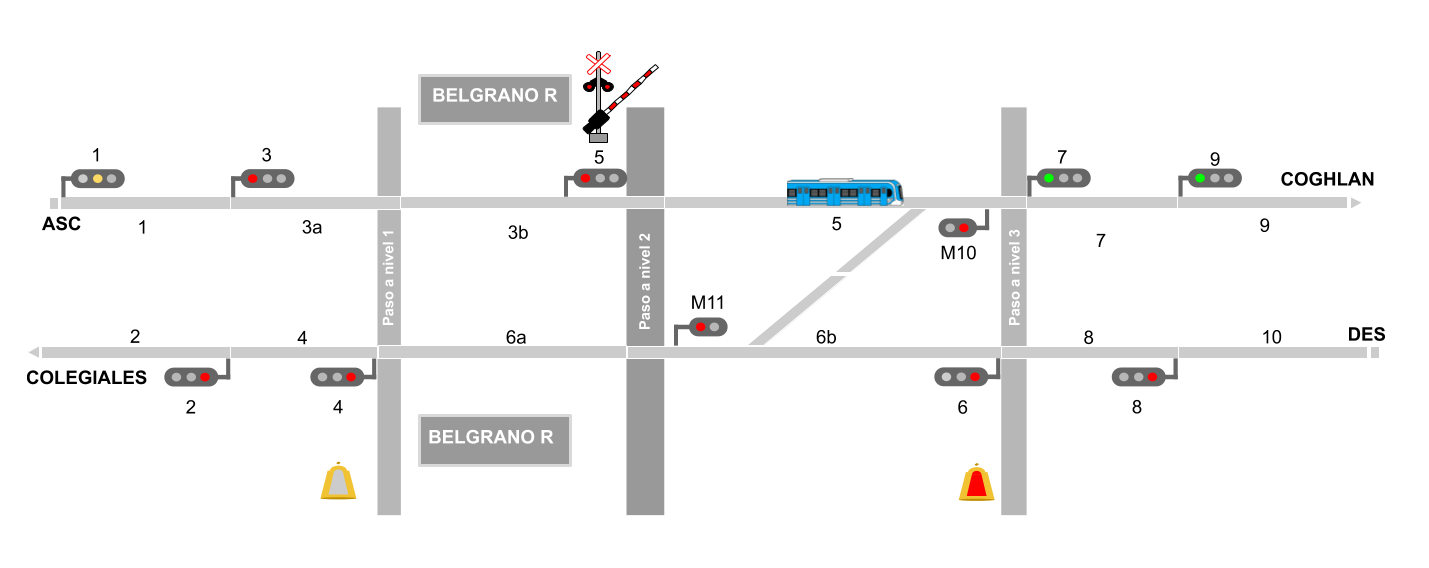
\includegraphics[scale=.27]{./Figures/Belgrano_R}
			\caption{Ejemplo de implementación de Belgrano R.}
			\label{fig:CESE_1}
		\end{figure}	
		
		%\vspace{5cm}
		
		A partir de esta experiencia se concluyó que es muy importante diseñar e implementar un método de trabajo que brinde reusabilidad, y que también sea escalable, de modo que se pueda aplicar en topologías más grandes y complejas. El método de trabajo a desarrollar debe ser tal que minimice la probabilidad y severidad de fallas humanas en el proceso de diseño y revisión.
				
		%Fue necesario garantizar no solo la reusabilidad, en el caso de locaciones de un tamaño similar a Belgrano R; sino que también su escalabilidad a topologías mas complejas. Una mayor cantidad de elementos ferroviarios implica una densidad mayor de circuitos lógicos, y estos a su vez repercuten en un crecimiento enormemente de la complejidad del desarrollo, mayor dificultad para implementar los ensayos y mayores chances de errores al extrapolar posibles fallas humanas a sistemas de mayor tamaño.
		
		%La solución a proponer no podía quedar sujeta a una única topología, ya que aun culminando el proyecto se corría el riesgo de que el tiempo empleado fuese desperdiciado si se cambiaban los requerimientos de forma abrupta. 
		
		Es por eso que, en el marco de la Maestría en Sistemas Embebidos, se marcó como un objetivo central el desarrollo de una herramienta capaz de generar automáticamente la solución electrónica de un sistema de enclavamiento ferroviario, a partir de una representación matemática única de cada topología. En la figura \ref{fig:Generacion} se muestra una imagen ilustrativa del proceso propuesto, en el que diversas topologías son procesadas e implementadas en forma automática en una plataforma FPGA.
				
		\begin{figure}[htbp!]
			\centering
			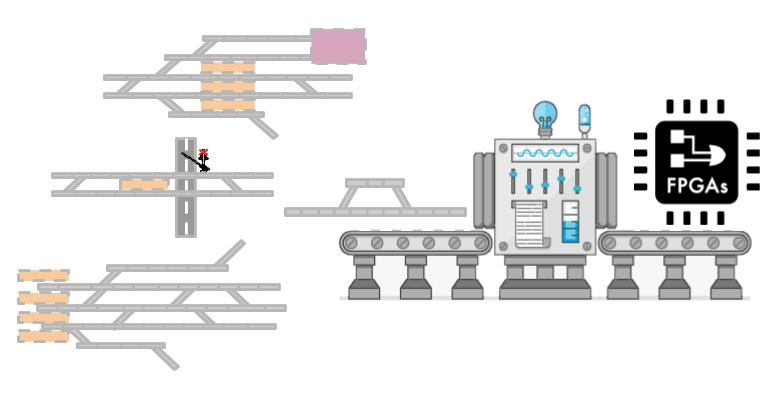
\includegraphics[scale=.45]{./Figures/Generacion}
			\caption{Proceso de generación automática de la solución electrónica.}
			\label{fig:Generacion}
		\end{figure}
		
		\vspace{10cm}
		
		% Spyder -> programa
		% Carpeta de archivos VHDL		
		% Carpeta de mapas generados
		% Captura de esquematico generado
		
		De esta manera, la solución desarrollada parte de cualquier red ferroviaria (figura \ref{fig:Spyder}), y mediante un analizador de redes ferroviarias, diseñado e implementado en el marco de este trabajo, determina qué función cumplirá cada elemento de la red y cuántos semáforos, de cuántos aspectos, en qué orientación y en qué ubicación deben utilizarse para que el sistema sea seguro.
		
		\begin{figure}[htbp!]
			\centering
			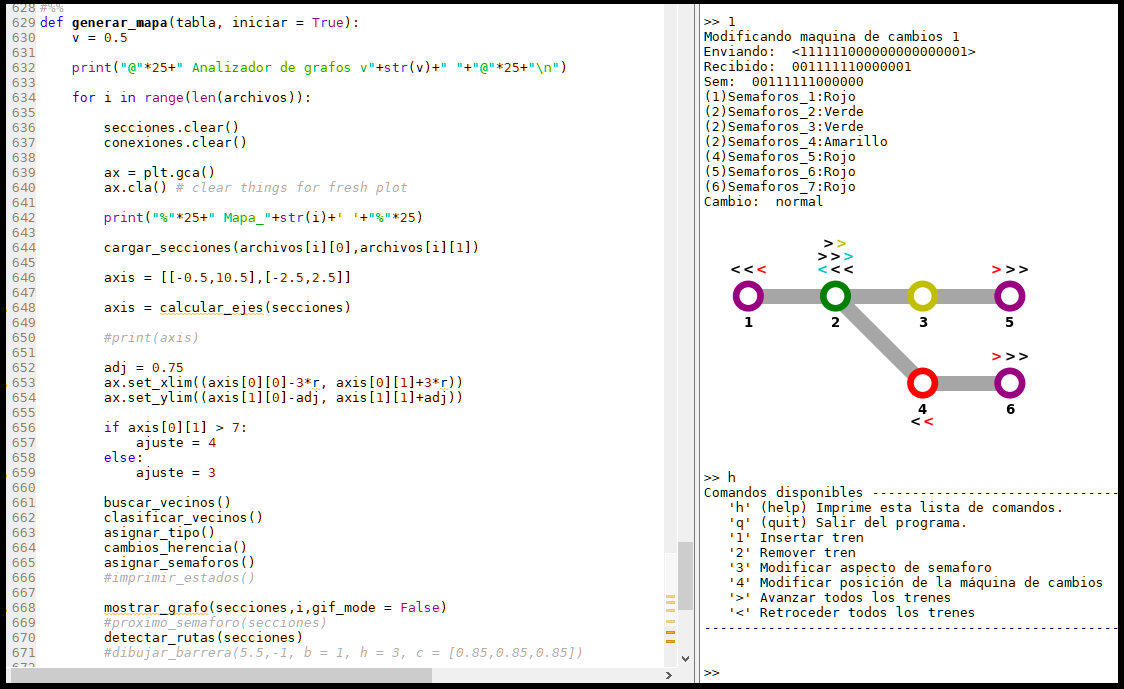
\includegraphics[scale=.4]{./Figures/Spyder}
			\caption{Analizador de redes ferroviarias desarrollado en Python.}
			\label{fig:Spyder}
		\end{figure}
				
		A continuación, en base a los semáforos insertados el analizador calcula todas las rutas posibles que admite esa red y genera automáticamente la solución electrónica para ser implementada mediante una FPGA. Puede verse en la figura \ref{fig:Archivos} un ejemplo de los archivos .vhdl generados automáticamente producto del análisis de una determinada red ferroviaria.		
		
		\begin{figure}[htbp!]
			\centering
			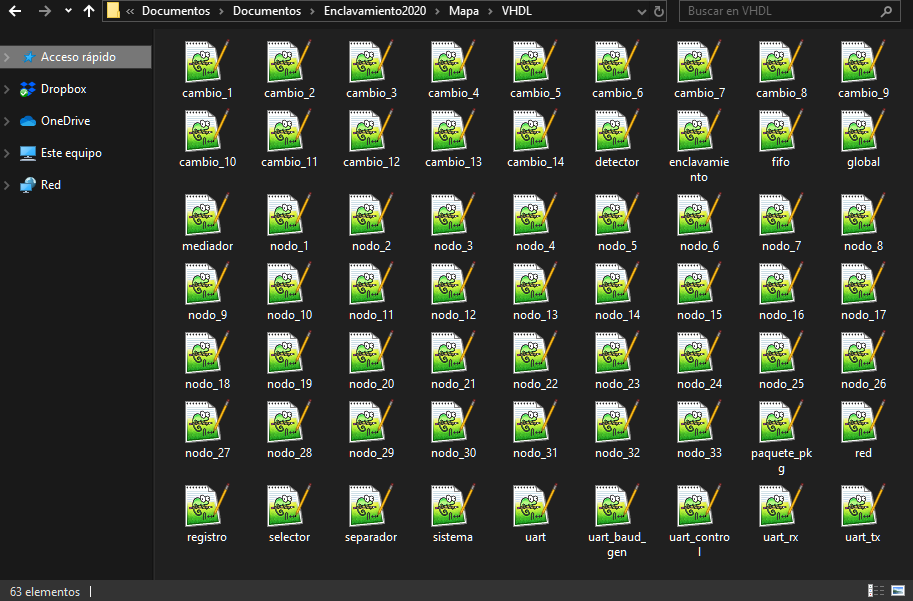
\includegraphics[scale=.5]{./Figures/Archivos}
			\caption{Archivos VHDL generados por el analizador de redes ferroviarias.}
			\label{fig:Archivos}
		\end{figure}
		
		De esta forma el sistema desarrollado puede procesar en cuestión de minutos decenas de topologías ferroviarias y generar las correspondientes implementaciones de la solución electrónica. Esto se ilustra en la figura \ref{fig:Topologias}. 
		
		\begin{figure}[htbp!]
			\centering
			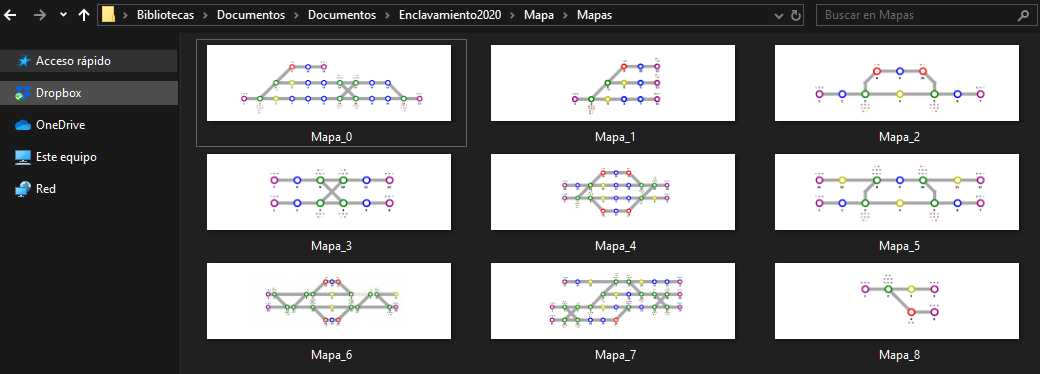
\includegraphics[scale=.5]{./Figures/Topologias}
			\caption{Ejemplos de algunas topologías luego de ser procesadas por el sistema desarrollado.}
			\label{fig:Topologias}
		\end{figure}
		
		En la figura \ref{fig:Esquematico} se muestra a modo de ejemplo la solución electrónica lista para ser implementada en una FPGA que corresponde a los archivos .vhdl ilustrados en la figura \ref{fig:Archivos}.
		
		\begin{figure}[htbp!]
			\centering
			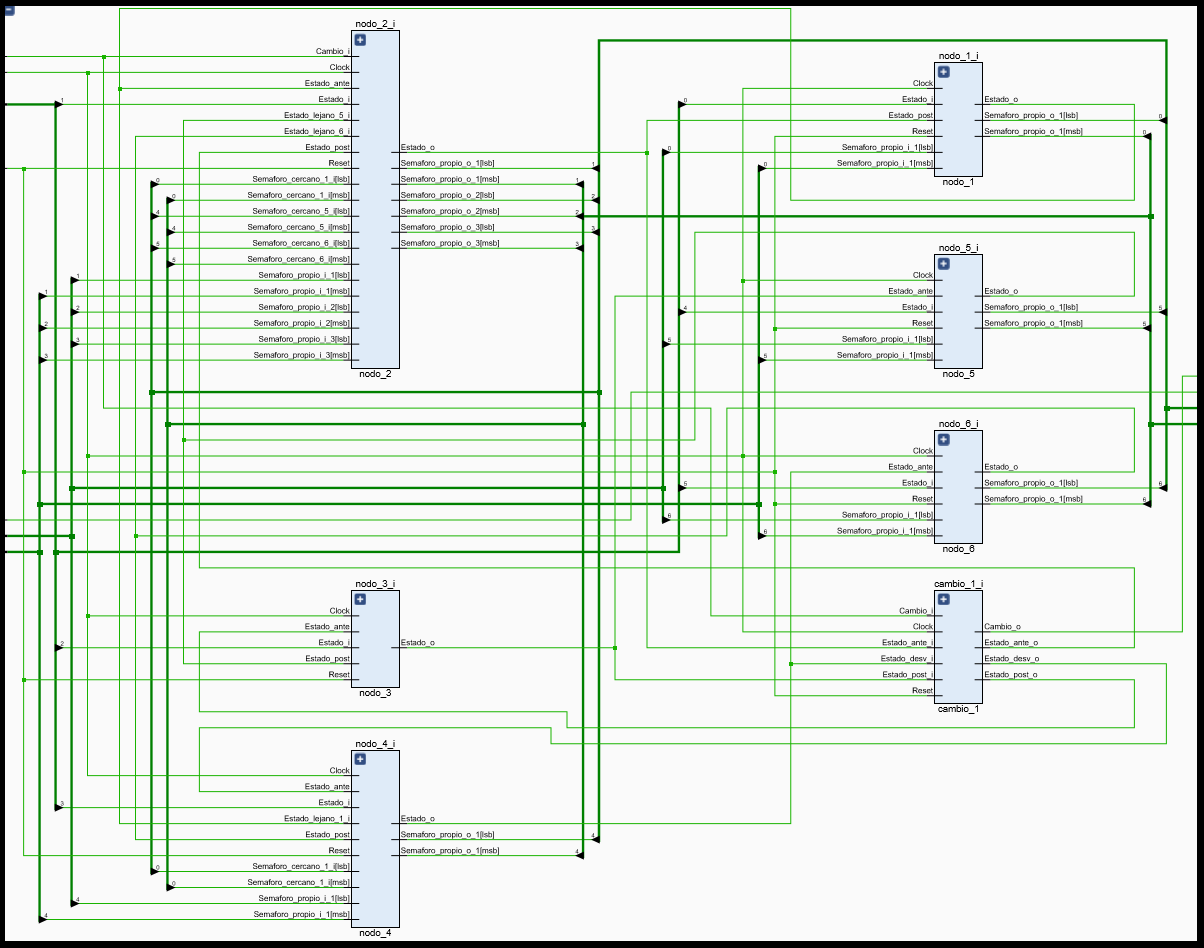
\includegraphics[scale=.45]{./Figures/Esquematico}
			\caption{Esquemático generado por el analizador de redes ferroviarias.}
			\label{fig:Esquematico}
		\end{figure}
		
		Para poder entender mejor el funcionamiento del sistema desarrollado es necesario introducir conceptos propios del mundo ferroviario y sus componentes involucrados. Estos se describen en la siguiente sección.

	\section{Elementos del señalamiento ferroviario}
	
		En este trabajo se reutilizan las mismas definiciones de los elementos ferroviarios presentadas en la memoria del Trabajo Final de la Carrera de Especialización en Sistemas Embebidos, ya que son las definiciones mas precisas que este autor pudo elaborar y el paso del tiempo no ha modificado su validez.
		
		La función del señalamiento ferroviario es evitar las colisiones entre trenes y los descarrilamientos. A continuación se describen los diferentes elementos que componente el señalamiento y que fueron modelados durante este trabajo.
		
		\subsection{Vías}
			
			Las vías férreas (figura \ref{fig:Via_eclisa}) consisten en el elemento esencial de la infraestructura ferroviaria y conforman el sitio por el cual se desplazan los trenes. Se encuentran separadas por una distancia fija que se mide desde sus caras internas y se denomina trocha.
			
			\begin{figure}[htbp!]
				\centering
				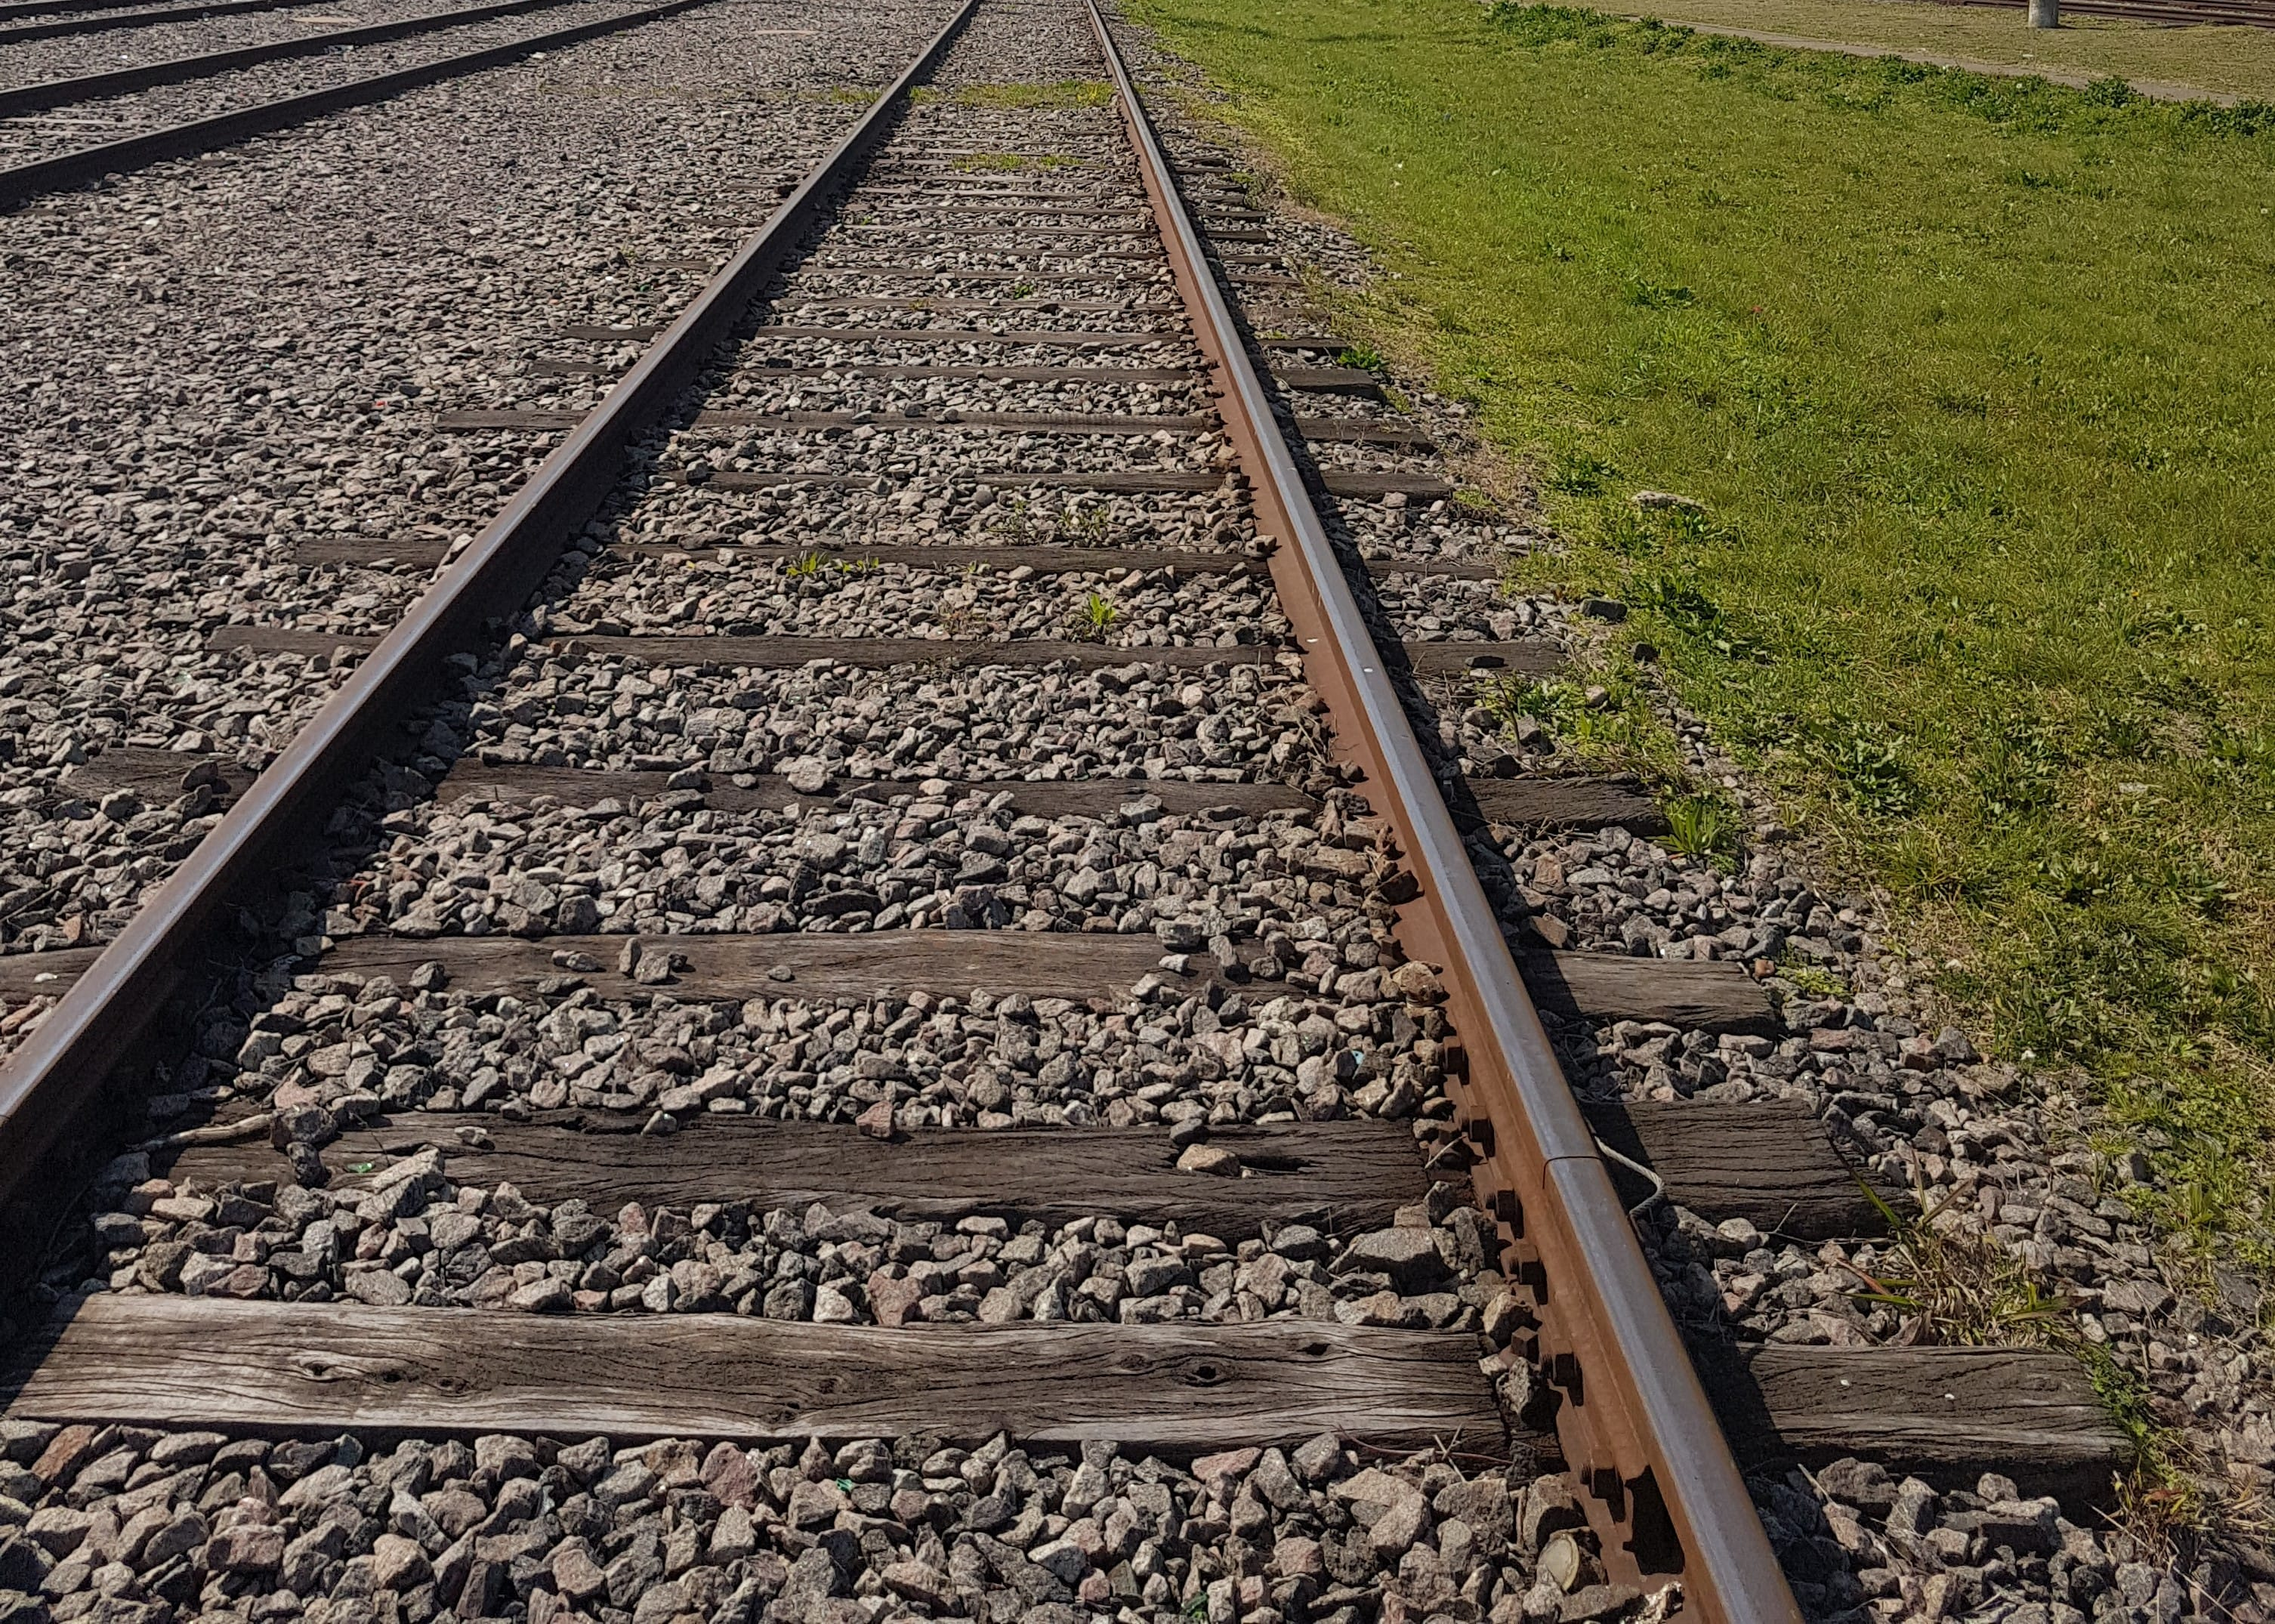
\includegraphics[scale=.07]{./Figures/Tramo_via}
				\caption{Tramo de vía ferroviaria.}
				\label{fig:Via_eclisa}
			\end{figure}	
			
			%\vspace{7cm}
			
			Las vías se dividen en secciones y por seguridad se establece que cada sección puede contener solo una formación por vez. Las mismas pueden tener largos variables en zonas urbanas de entre 500 a 1000 metros en zonas rurales. 
			
			Cada vía puede ser clasificada en dos grupos: vías ascendentes o vías descendentes. Las ascendentes son aquellas por las que los trenes circulan únicamente en la dirección del kilometraje en sentido creciente. Las descendentes son aquellas por las que los trenes circulan únicamente en la dirección del kilometraje en sentido decreciente\cite{RITO}. El kilómetro 0 es la estación principal de la línea ferroviaria, como por ejemplo: Plaza Constitución (para la línea Roca), Once de septiembre (para la línea Sarmiento) o Retiro (para las líneas Mitre y San Martín).
			
			Existen vías de maniobra que pueden ser tanto ascendentes como descendentes. Estas vinculan, mediante un cambio de vías, una sección ascendente con otra descendente, en la cual los trenes deben circular a una velocidad reducida.
			
		\subsection{Semáforos ferroviarios}
			
			El sistema de enclavamientos utiliza los semáforos ferroviarios para indicarle al conductor del tren si puede o no acceder al próximo tramo de vías y a qué velocidad se le permite circular; esto, por medio del color del semáforo, denominado aspecto. A diferencia de los semáforos vehiculares, en los que cada color es alternado por otro de la secuencia rojo-amarillo-verde en función del tiempo, los semáforos ferroviarios cambian su aspecto en función de los eventos de los tramos siguientes.
					
			En la figura \ref{fig:Sem_3Aspectos} se presenta un esquema de señales de tres aspectos, que es el tipo de semáforo que se utiliza en la gran mayoría de las líneas ferroviarias.
						 	
			 \begin{figure}[htbp!]
				\centering
				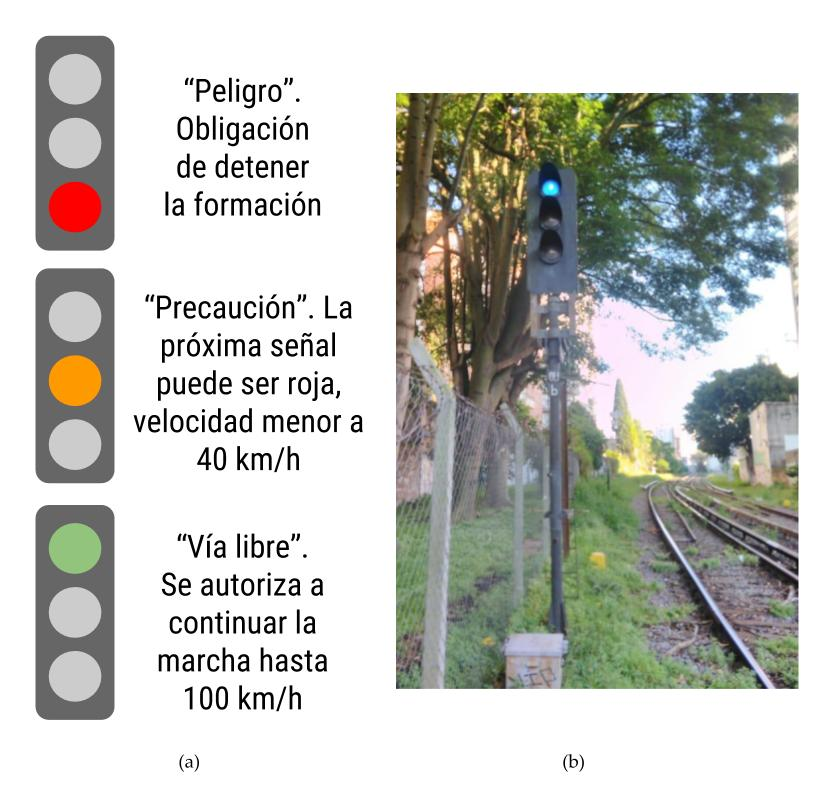
\includegraphics[scale=.28]{./Figures/Sem3}
				\caption{(a) Semáforo de tres aspectos\\(b) Semáforo doble de tres aspectos (Estación Olivos).}
				\label{fig:Sem_3Aspectos}
			\end{figure}
			
			Otra diferencia fundamental es que no todos los semáforos ferroviarios poseen tres aspectos. Los semáforos de maniobras constan de solo dos, amarillo (precaución) y rojo (prohibido avanzar), y algunas líneas como la Línea Roca utilizan semáforos de cuatro aspectos.	
			
			En la figura \ref{fig:Sem_2Aspectos} se visualizan los semáforos de dos aspectos. Se utilizan en cambios de vías donde, por su peligrosidad, solo se podrían permitir aspectos rojos y amarillos.
			 
			 \begin{figure}[htbp!]
				\centering
				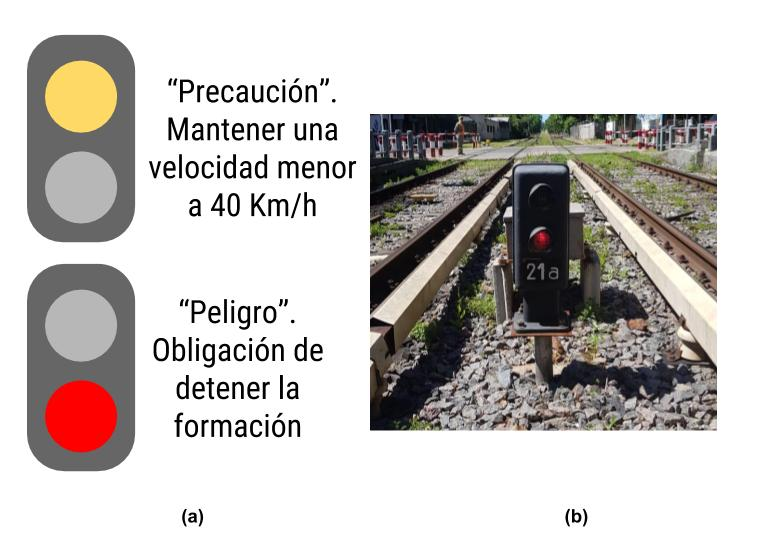
\includegraphics[scale=.28]{./Figures/Sem2}
				\caption{(a) Semáforo de dos aspectos\\(b) Semáforos de cruce de vías (Estación Lavallol).}
				\label{fig:Sem_2Aspectos}
			\end{figure}				
			
			\vspace{10cm}
			
			Los semáforos de cuatro aspectos son utilizados en la Línea Roca y poseen un doble amarillo antes del amarillo simple, para permitir así tramos de vías mas cortos en forma segura. Como no son objeto de estudio del presente trabajo, no serán explicados aquí.
		
		\subsection{Circuito de vías}
		\label{CVs}
		
			Para poder determinar si un tramo de la vía se encuentra ocupado o libre se utilizan los circuitos de vías. Estos constituyen componentes electrónicos que imponen una tensión conocida entre los rieles, y cuando un tren se posiciona sobre esa sección provoca un cortocircuito que es detectado por el circuito. En la figura \ref{fig:Ocupacion} se ejemplifica la ocupación de las secciones por una formación (modelada con un 0) y la ausencia de formación (modelada con un 1).
			
			\begin{figure}[h]
				\centering
				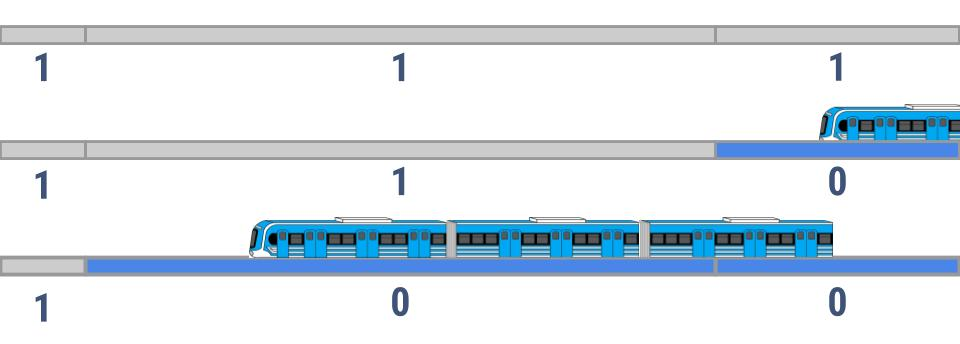
\includegraphics[scale=.4]{./Figures/Ocupacion}
				\caption{Ocupación de las secciones de vías.}
				\label{fig:Ocupacion}
			\end{figure}
			
			%\vspace{7cm}
			
			Si el tramo de vía no tiene ninguna formación ocupándolo, el señalamiento indicará un aspecto verde o amarillo según el estado de ocupación del tramo siguiente. Si la formación ocupa la sección, el señalamiento cambiará su aspecto a rojo para indicar que no puede ingresar ninguna otra formación, a fin de evitar colisiones. Por seguridad también se establecerá a rojo el semáforo anterior y a amarillo el anterior a este (doble recubrimiento), tal como se ilustra en la figura \ref{fig:Recubrimiento}.			
					
			\begin{figure}[h]
				\centering
				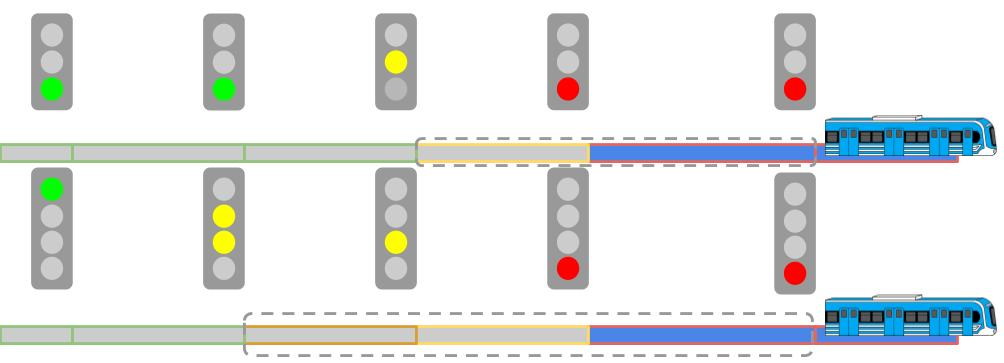
\includegraphics[scale=.4]{./Figures/Recubrimiento}
				\caption{Estado de los aspectos ferroviarios según la ubicación del tren.}
				\label{fig:Recubrimiento}
			\end{figure}			
			
			Si la alimentación es interrumpida o si el cableado sufre alguna falla, entonces el sistema asumirá que hay un tren en las vías y los semáforos se pondrán en aspecto rojo para que las formaciones cercanas detengan su marcha y las barreras de los pasos a nivel desciendan. A este principio se lo denomina \textit{fail-safe}\footnote{\textit{fail-safe}: falla segura.}. Es decir, si por alguna razón algo falla, el sistema adopta la condición mas restrictiva, mitigando la posibilidad de una situación peligrosa. 		
			
		\subsection{Pasos a nivel}
		
			La intersección de una ruta vehicular o peatonal con la vía férrea se denomina paso a nivel. El sistema de control de la barrera mantiene el brazo de esta en alto para permitir la circulación vehicular, como se puede ver en la figura \ref{fig:Paso_a_nivel}. Si un tren ocupa las secciones amarillas de la figura \ref{fig:Paso_a_nivel} se desenergiza la barrera y comienza a descender el brazo por efecto de la gravedad. Cuando se ocupen las secciones azules de la figura \ref{fig:Paso_a_nivel}, entonces se accionará la alarma sonora para alertar a los peatones que deben permanecer en el laberinto contiguo a la vía, cuya función es forzar a los peatones a mirar a ambos lados antes de cruzar el paso a nivel.			
			
			\begin{figure}[h!]
				\centering
				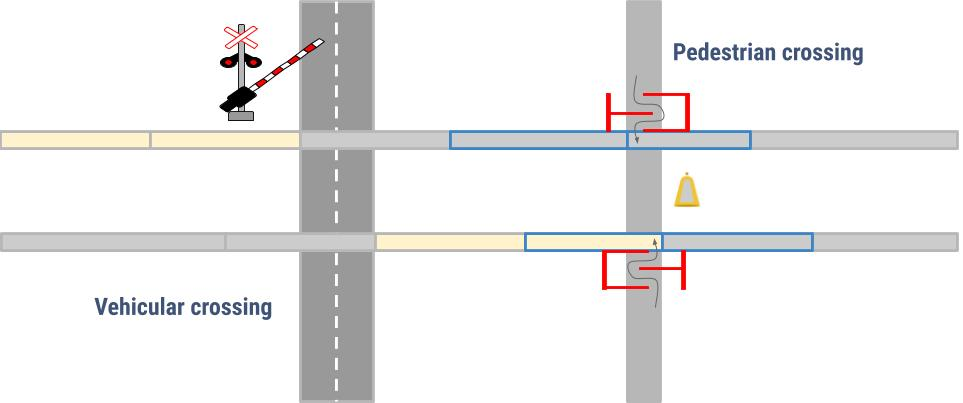
\includegraphics[scale=0.4]{./Figures/Paso a nivel}
				\caption{Pasos a nivel vehicular y peatonal sobre vía férrea.}
				\label{fig:Paso_a_nivel}
			\end{figure}
			%\vspace{5cm}
			
			Solo cuando la barrera baja, el tren tiene permitido avanzar sobre el cruce, siendo el paso a nivel un sector de altísimo riesgo.
			
			Al desocuparse las las secciones amarillas, la barrera vuelve a energizarse y se sitúa en estado alto nuevamente, a la espera de otro tren para reiniciar el proceso descripto.
						
			Se debe destacar que el mismo proceso de descenso de la barrera ocurrirá si esta se desenergiza por una falla eléctrica y/o pérdida de alimentación. Es decir, el sistema asumirá el estado mas seguro ante cualquiera de los mencionados fallos, siguiendo el principio de falla segura.
		
		\subsection{Máquina de cambios}
			
			Una máquina de cambios (figura \ref{fig:Cambio}) es un mecanismo utilizado para permitir el paso de las formaciones de una vía a una ramificación del recorrido principal. Esto se realiza mediante el movimiento de la aguja del cambio (riel móvil) hacia su respectiva contraaguja (riel fijo) hasta obtener un adecuado acoplamiento que permita la circulación de la formación.
			
			\begin{figure}[h!]
				\centering
				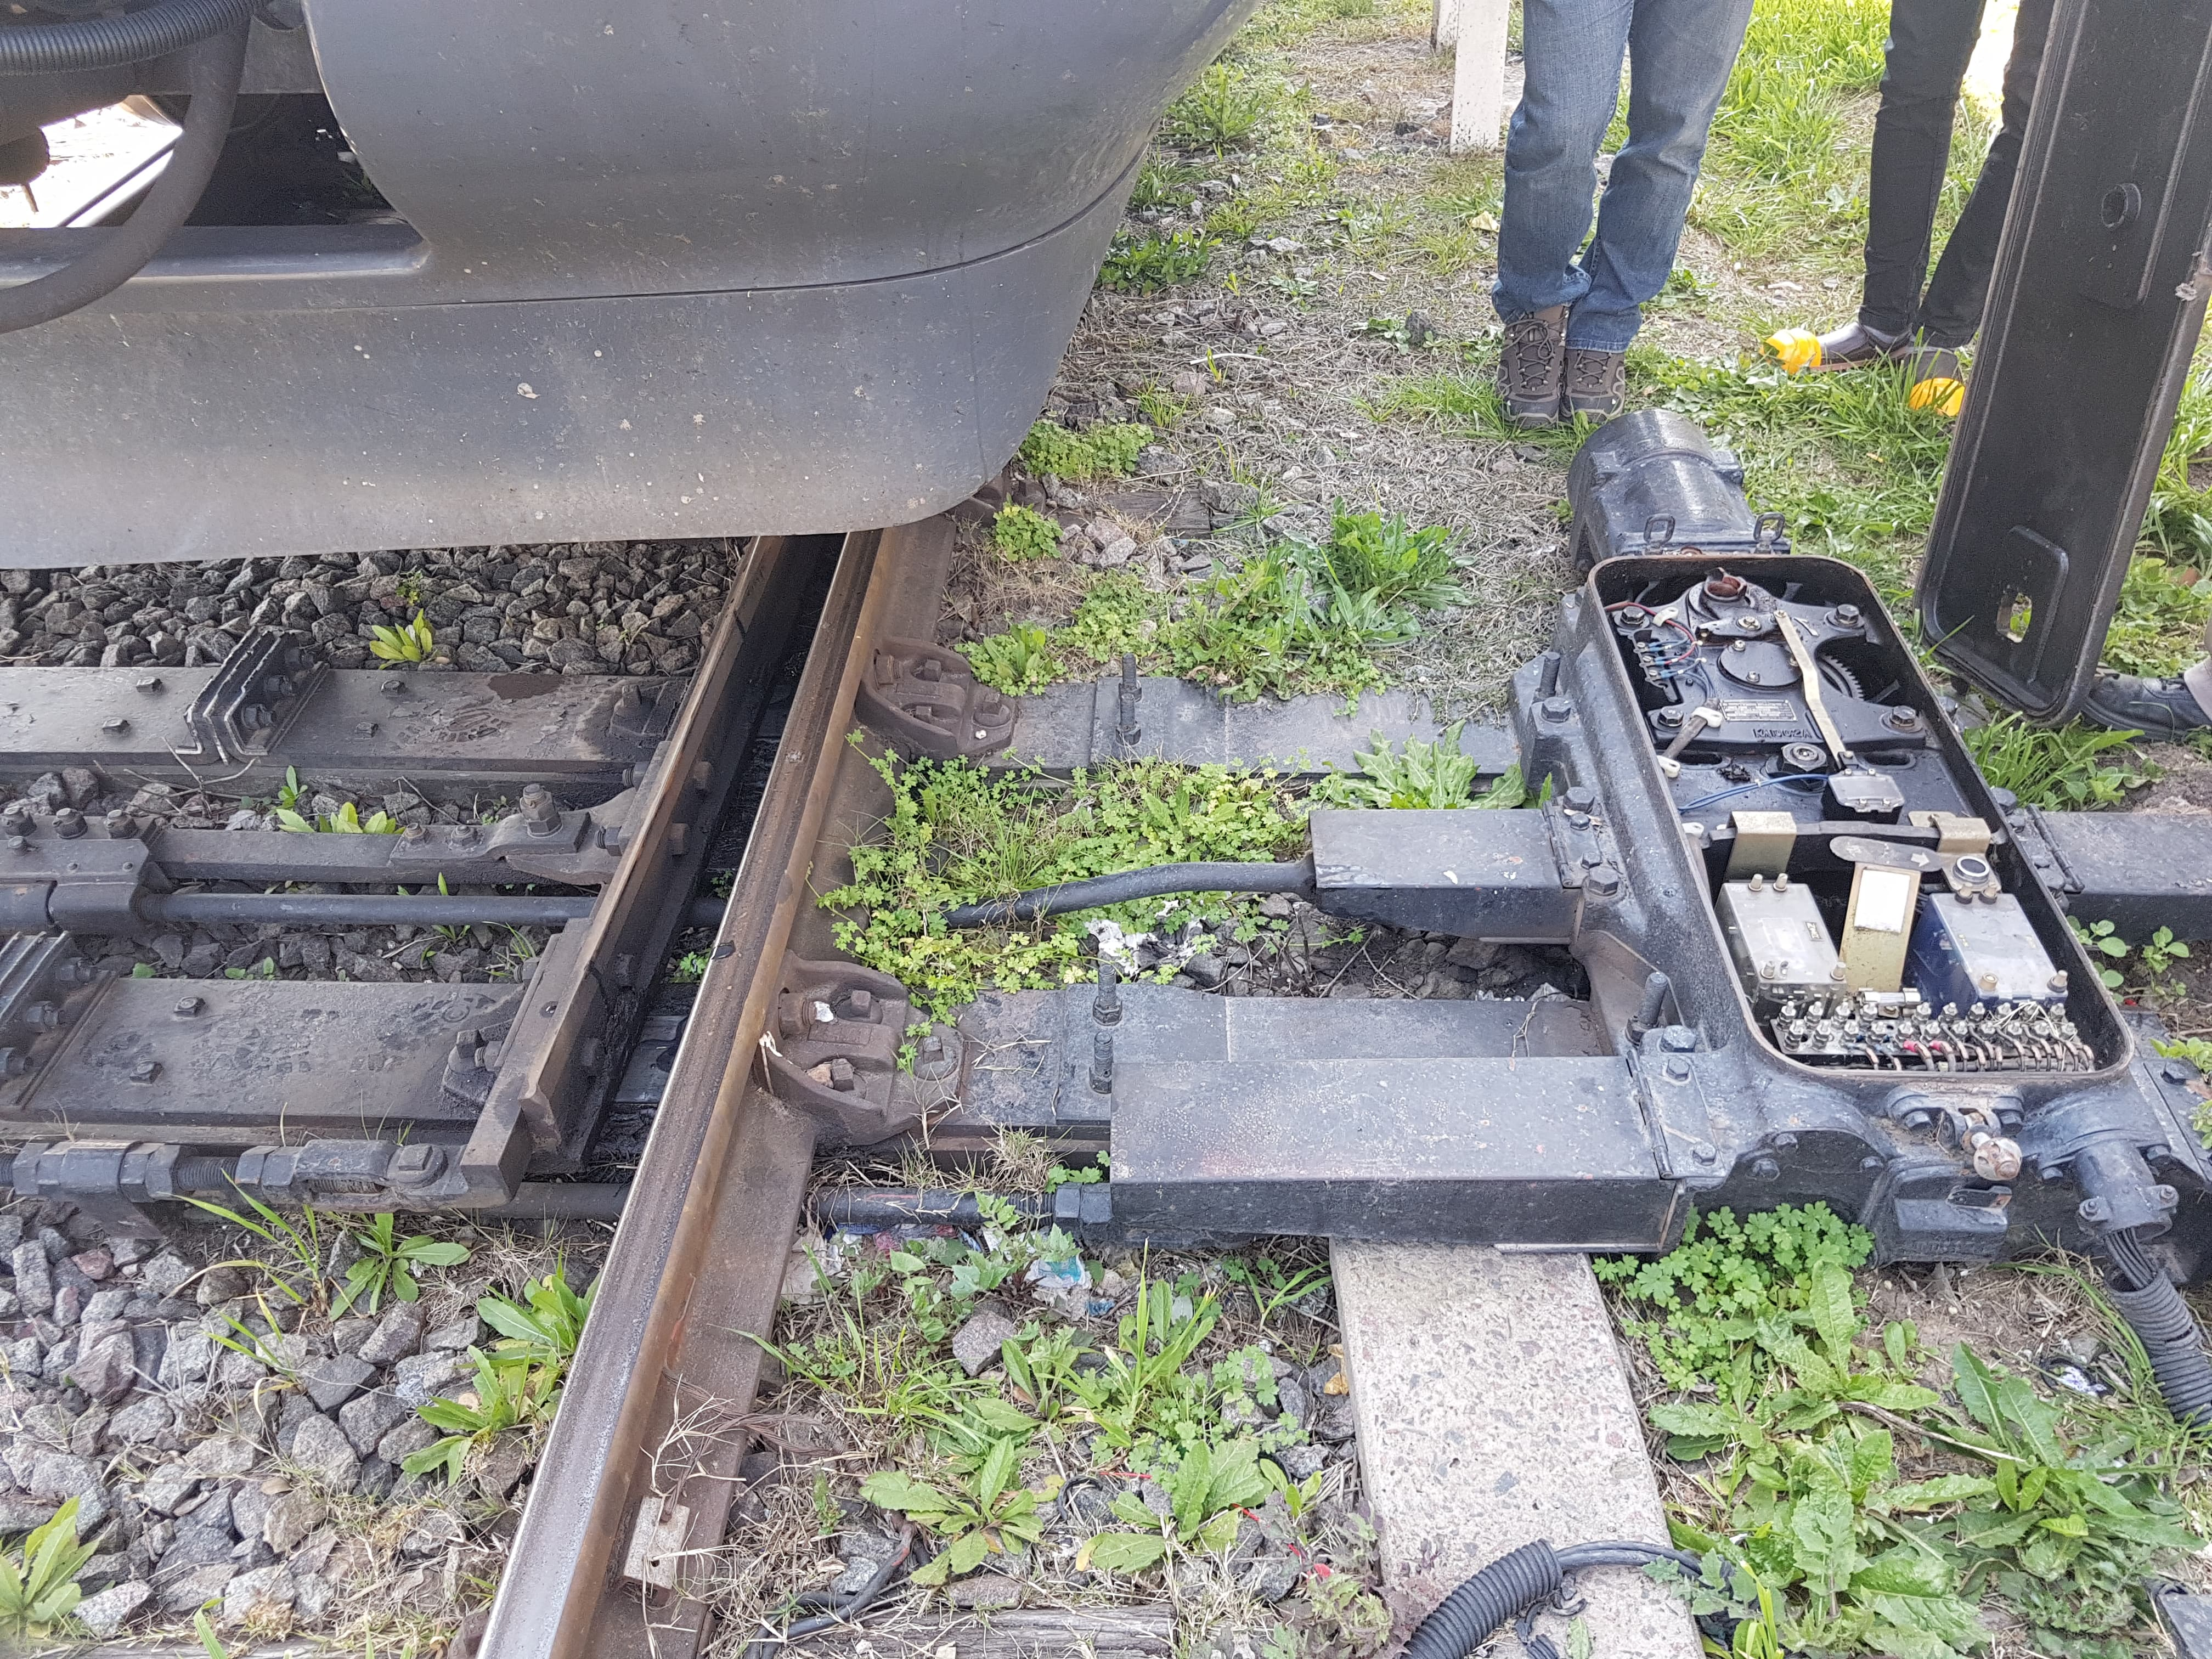
\includegraphics[scale=.06]{./Figures/Cambio}
				\caption{Máquina de cambios de Lavallol (Línea Roca).}
				\label{fig:Cambio}
			\end{figure} 
			
			\vspace{7cm}
			
			En la figura \ref{fig:Cambios_2} se muestra el cambio de vía de la estación Matheu de la Línea Mitre. Se observa que según sea la posición de la máquina de cambios, el tren puede continuar en la misma vía o hacer el cambio a la otra vía.
			
			\begin{figure}[h!]
				\centering
				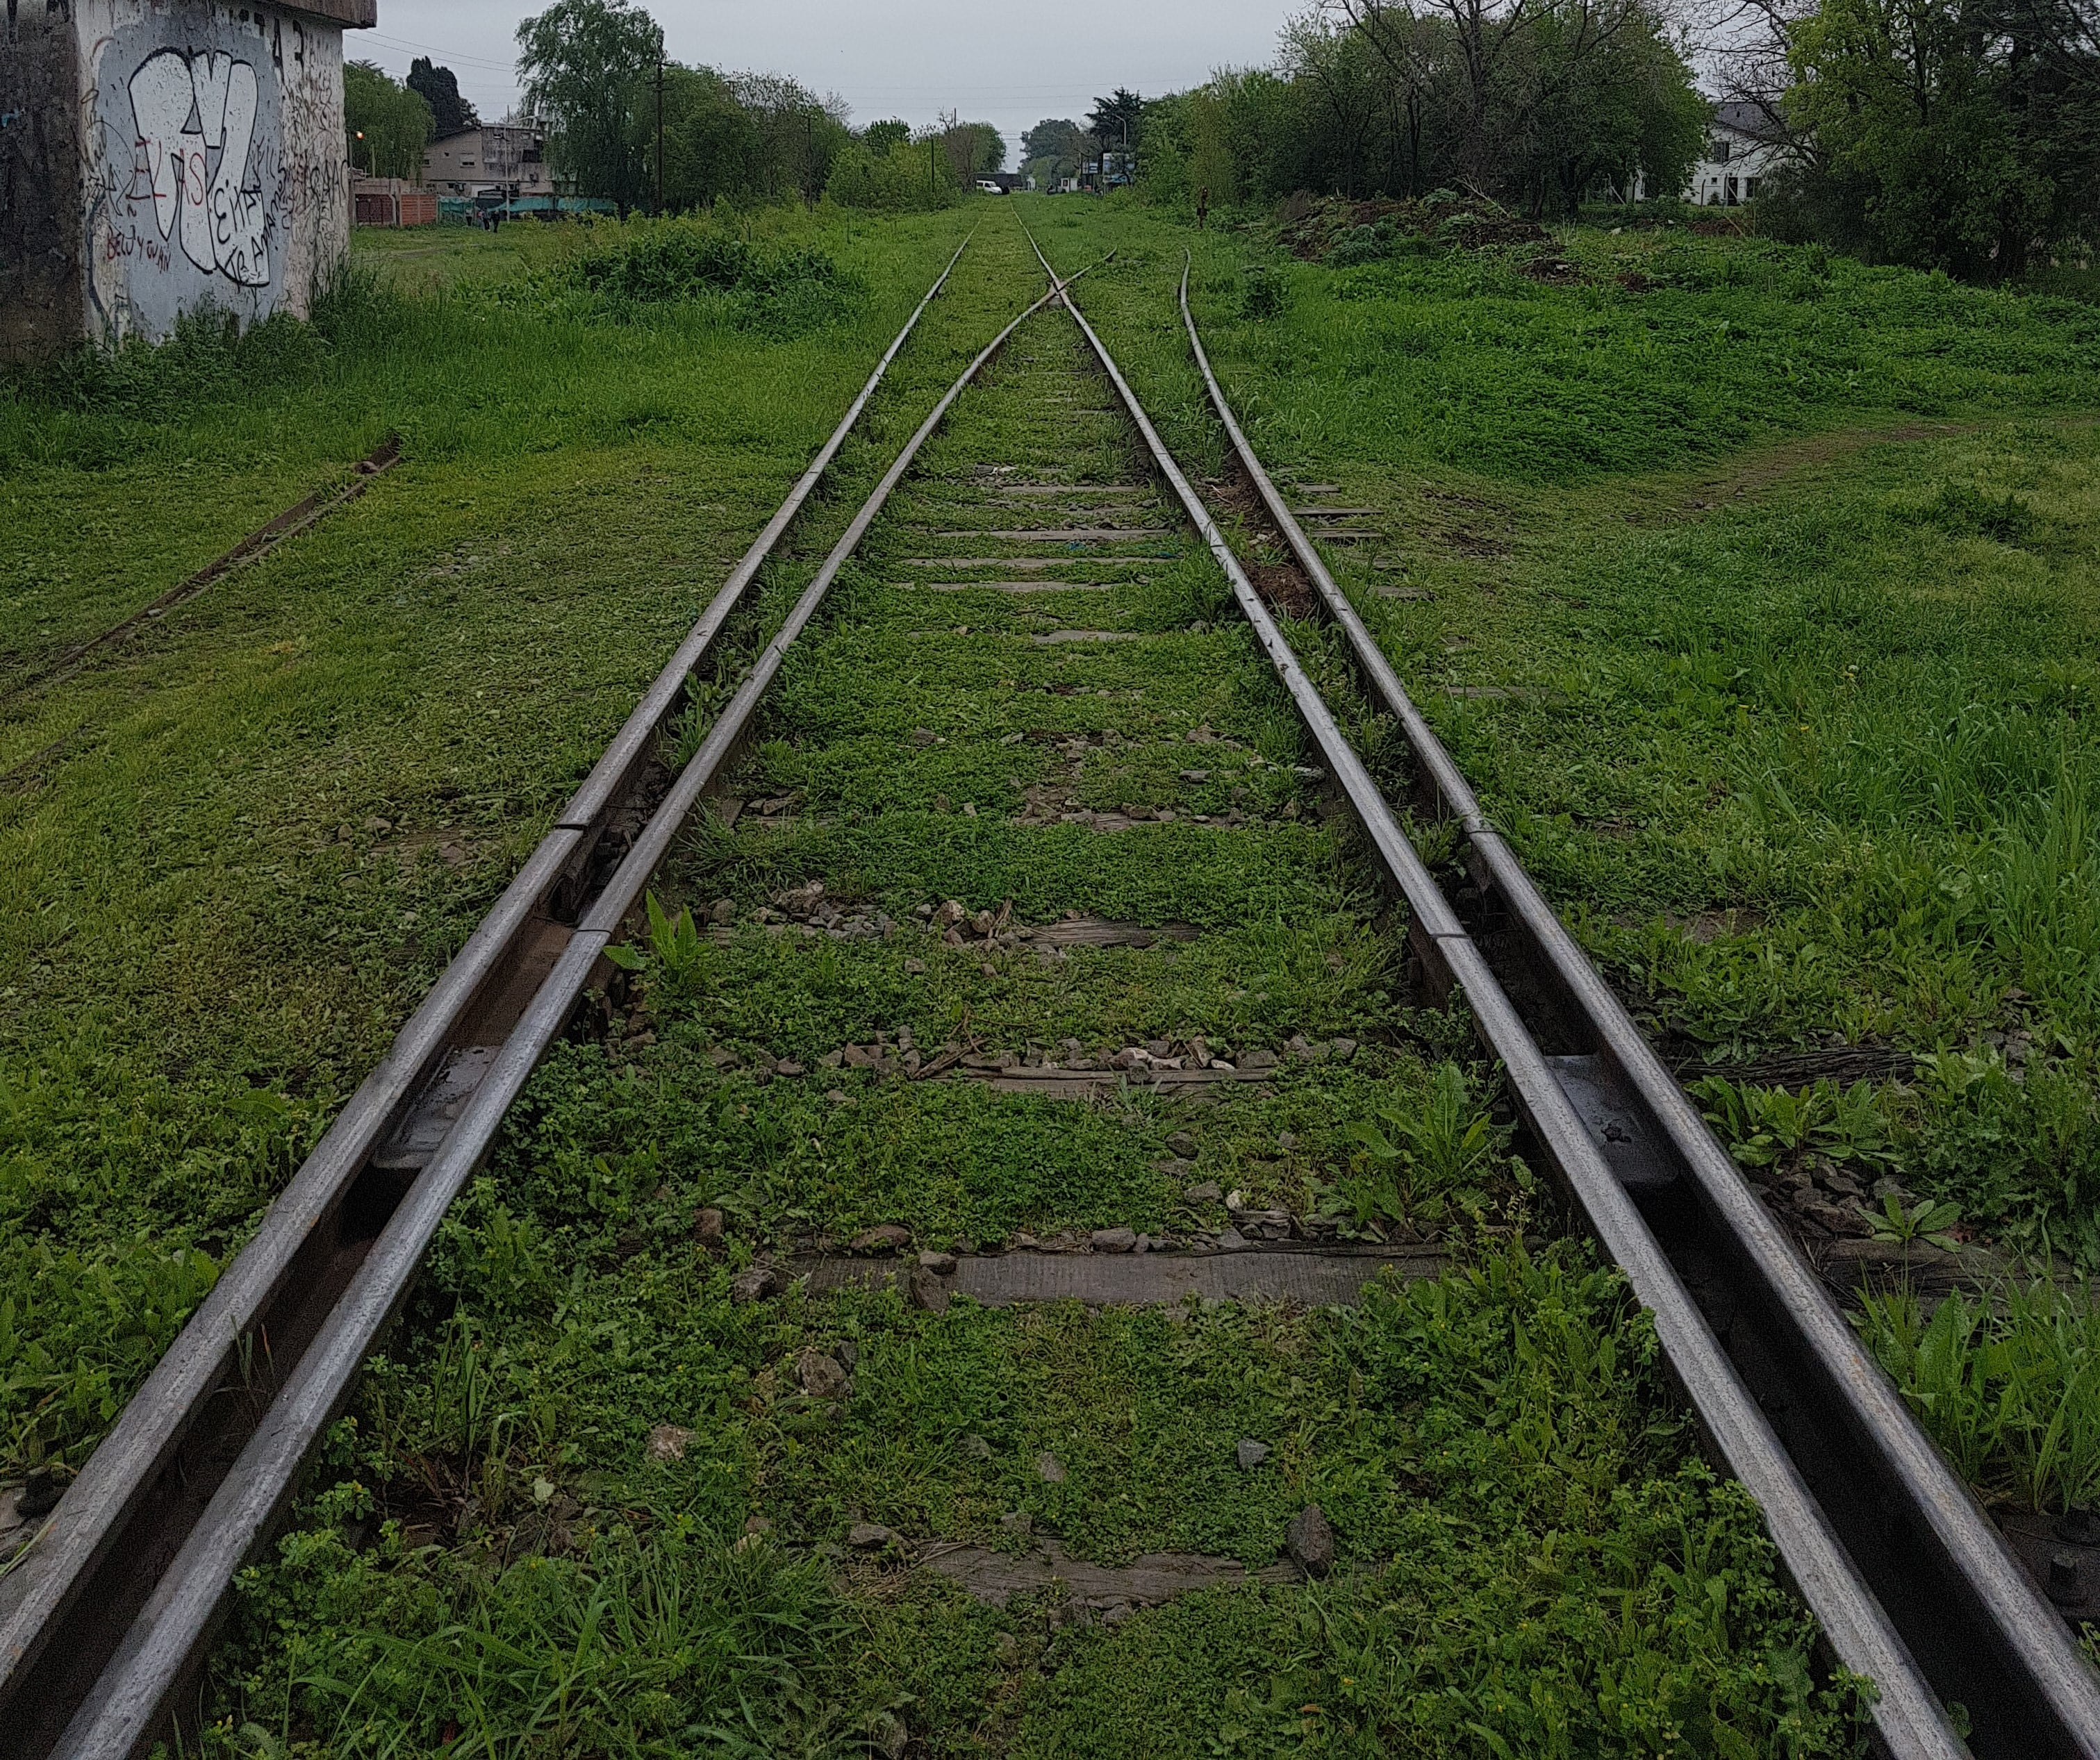
\includegraphics[scale=.1]{./Figures/Cambios_2}
				\caption{Cambio de vías de estación Matheu (Línea Mitre).}
				\label{fig:Cambios_2}
			\end{figure} 
		
			En la figura \ref{fig:Cambios} se muestran las posiciones que puede adoptar el cambio. En la posición normal los trenes pueden circular de forma directa, en paralelo, por la vía principal en sentidos opuestos. En la posición reversa, en cambio, se permite el intercambio de trenes de una rama principal a otra en sentido opuesto o a una ramificación secundaria de la red.
			
			\begin{figure}[h!]
				\centering
				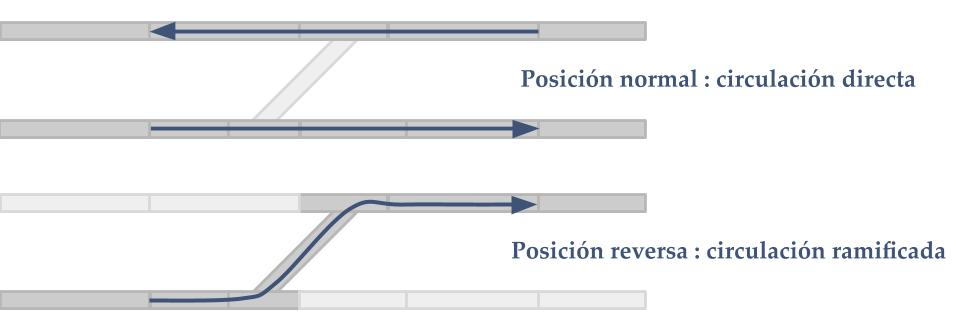
\includegraphics[scale=.4]{./Figures/Cambios}
				\caption{Posiciones normal e inversa del cambio.}
				\label{fig:Cambios}
			\end{figure} 	
					
	\section{Sistema de enclavamientos}

		A modo de ejemplo se ilustra en la figura \ref{fig:Bypass} un sistema de cambios en una vía simple con \emph{bypass}. Este permite que dos formaciones puedan cruzarse en sentidos opuestos sin colisionar.
	
		\begin{figure}[h!]
			\centering
			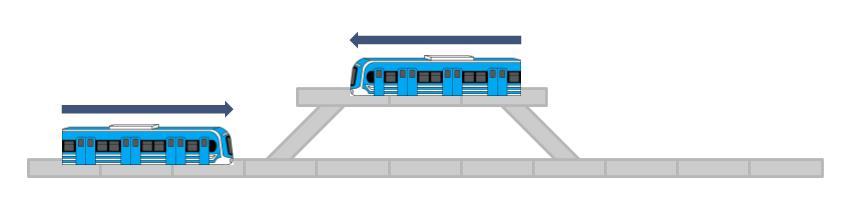
\includegraphics[scale=.45]{./Figures/Bypass_2}
			\caption{Vía simple con \textit{bypass}.}
			\label{fig:Bypass}
		\end{figure}
		%\vspace{5cm}
			
		Para evitar la colisión, se requiere un control seguro que evite que las formaciones avancen hacia secciones ya ocupadas por otras. También debe evitar que las formaciones avancen sobre los cambios cuando estos aún no han terminado de posicionarse en su lugar, lo que provocaría descarrillamientos. A este control se lo denomina sistema de enclavamiento y en definitiva impide que se produzcan las configuraciones no seguras y controla los semáforos que habilitan o no los itinerarios de las formaciones.		
					 
	 	Una falla en un enclavamiento puede poner en peligro cientos de vidas humanas y generar gastos considerables. Por lo tanto, en el diseño del sistema de enclavamiento se deben cumplir estrictos parámetros de fiabilidad, disponibilidad, mantenibilidad y seguridad (RAMS).
	 	
	 	Lamentablemente, los sistemas de enclavamientos en Argentina son en su mayoría mecánicos, de comienzos del siglo XX, y otra cantidad considerable son electromecánicos, de mas de 40 años de antiguedad. Muchos de ellos ya han agotado su vida útil y deben ser reemplazados. Otros, en cambio, han estado en desuso por años y necesitan ser repuestos, pero solo una docena de empresas en el mundo realizan el diseño del sistema y los costos para un bypass simple rondan las decenas de millones de dólares. Por esto, es importante contar con sistemas electrónicos de diseño y fabricación nacional.

		Además, existen diferentes lugares donde aún resta instalar este tipo de sistemas, por lo que su implementación constituye una necesidad real para el desarrollo de la infraestructura ferroviaria de señalamiento en Argentina.		
	
	\section{Tipos de enclavamientos}
		
		A continuación se presentan distintas tecnologías de implementación de enclavamientos en orden cronológico de invención.
		
		\subsection{Enclavamientos mecánicos}
			
			A comienzos del siglo XX se implementaron los sistemas de enclavamientos mediante soluciones mecánicas. Utilizaban palancas como las que se visualizan en la figura \ref{fig:Mecanico} para comandar los cambios de vías y semáforos.
	
			\begin{figure}[htbp!]
				\centering
				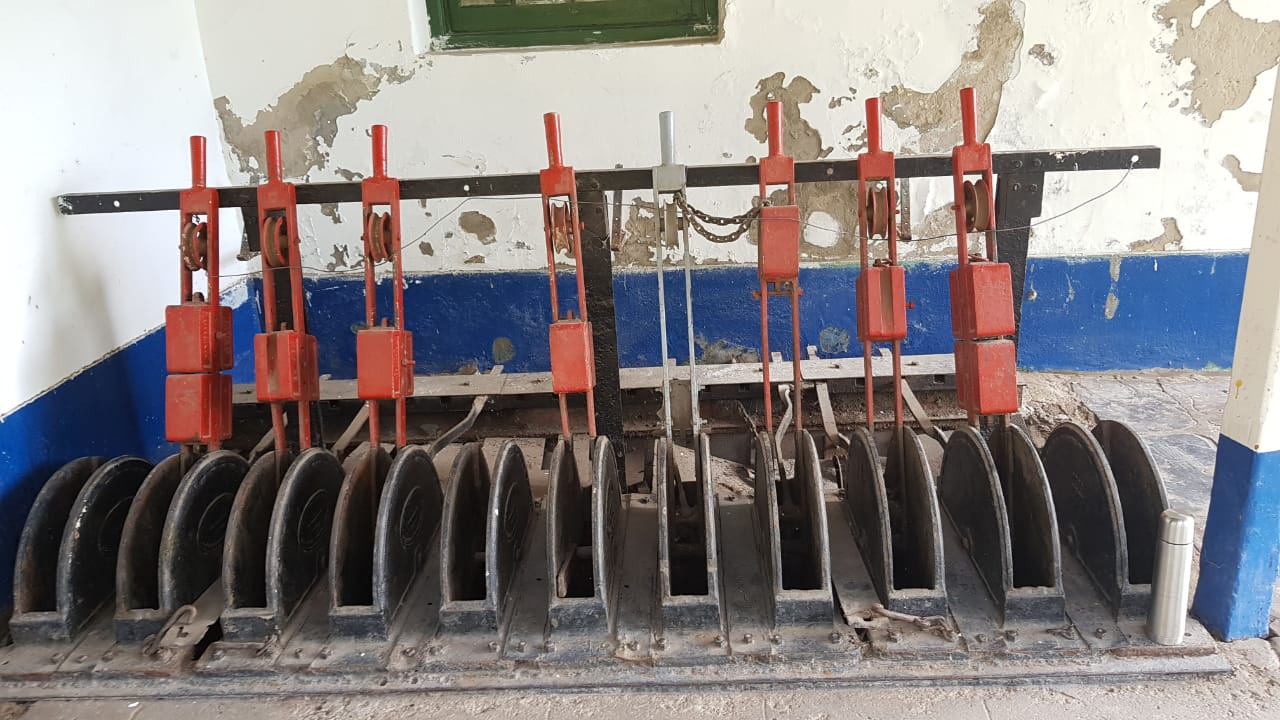
\includegraphics[scale=.27]{./Figures/Mecanico}
				\caption{Sistema enclavamiento mecánico en la estación de Chascomús, hoy convertida en museo.}
				\label{fig:Mecanico}
			\end{figure}

			Una vez que se constituye una configuración de posiciones de palancas que habilitan un trayecto, estas quedan <<enclavadas>> mecánicamente. Es decir, su posición se bloquea y no es físicamente posible cambiarla. A medida que se van moviendo ciertas palancas, las demás que pudieran representar situaciones no seguras quedan enclavadas, y solo se pueden mover aquellas cuyo accionamiento representa una situación segura. De esa manera se garantiza que no se generarán configuraciones tales que las formaciones colisionen entre sí.
			
			Las tecnologías mas modernas heredaron el término <<enclavamiento>>, aunque ya no se tengan palancas enclavadas en posiciones fijas.
		
		\subsection{Enclavamientos electromecánicos}
			
			A mediados del siglo XX se desarrolló el sistema de enclavamiento electromecánico. Su funcionamiento se basa en relés (figura \ref{fig:Reles}) y circuitos de vía, de forma tal de poder detectar la presencia de un tren y comandar tanto las señales como las barreras de los pasos a nivel.
				
			\begin{figure}[htbp!]
				\centering
				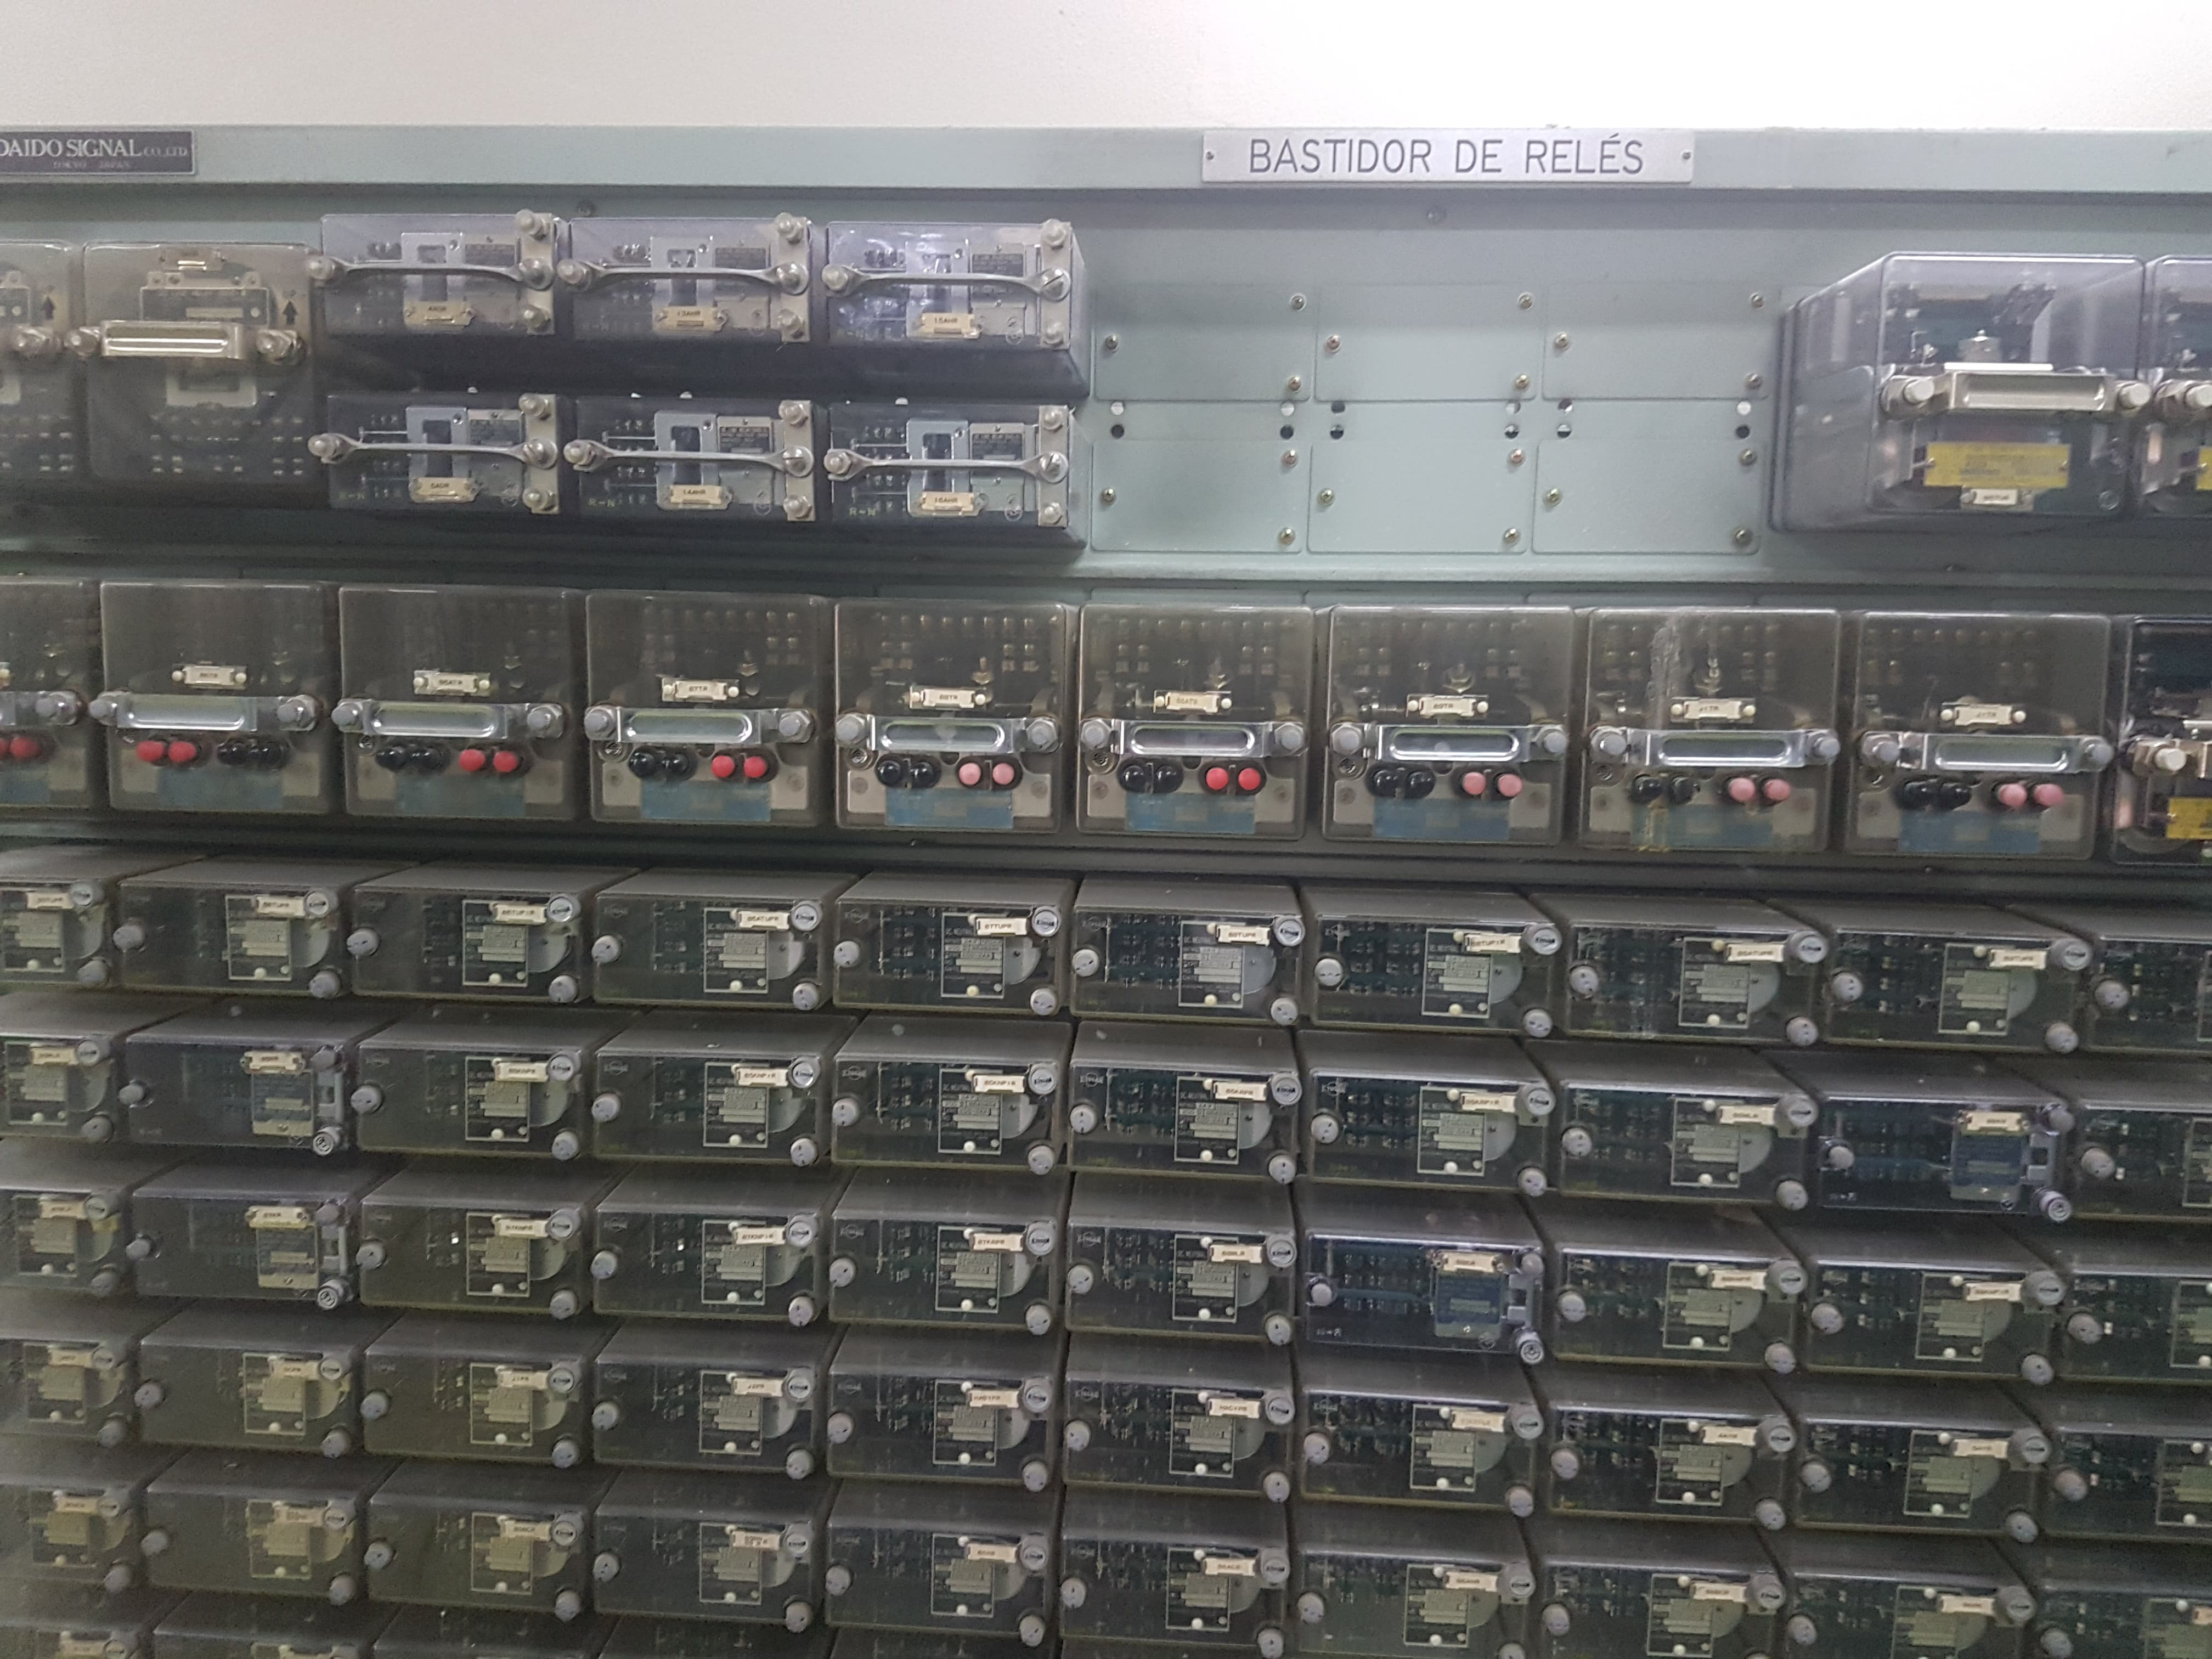
\includegraphics[scale=.08]{./Figures/Reles}
				\caption{Bastidor de relés de estación Lavallol (Línea Roca).}
				\label{fig:Reles}
			\end{figure}
		
			\vspace{7cm}
			
			Los sistemas de enclavamiento electromecánicos son comandados por un operario mediante un panel de control (figura \ref{fig:Electromecanico}). El operario solicita al sistema de enclavamiento las rutas que el conductor ferroviario necesita para circular. El sistema permitirá solo la operación de cambio de vías seguras. En caso contrario, se tendrán las salidas <<enclavadas>> y el sistema de enclavamiento impedirá mediante los semáforos el avance de la formación hasta que pueda realizarse el cambio en forma segura.
		
			\begin{figure}[h!]
				\centering
				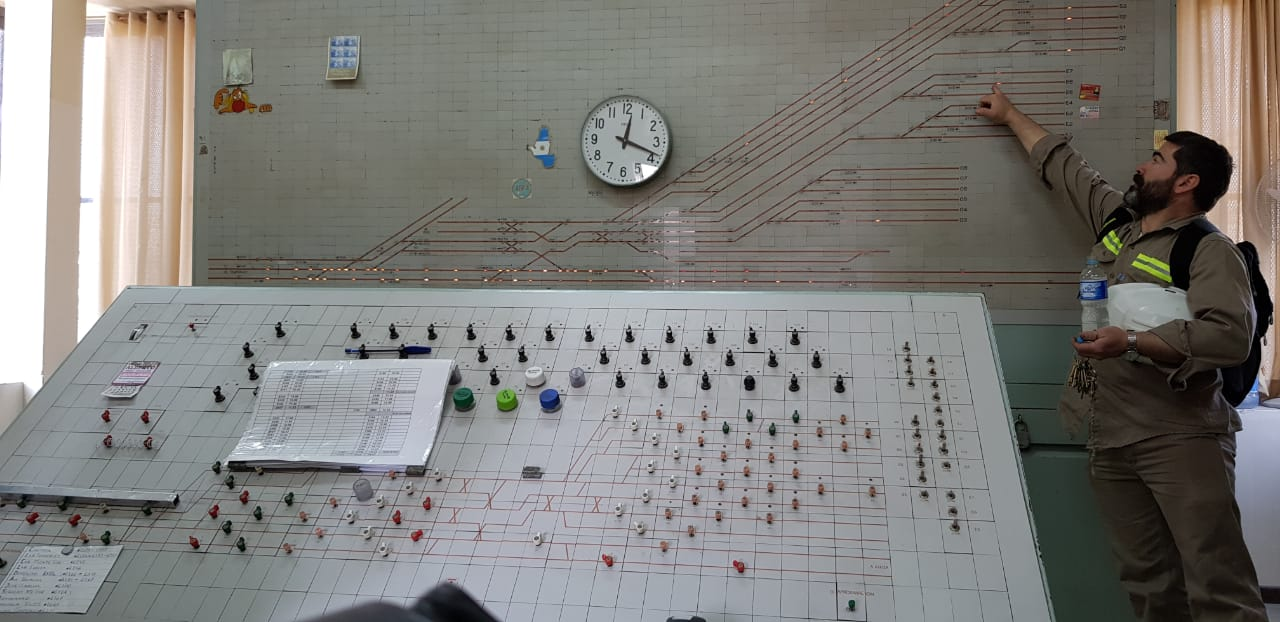
\includegraphics[scale=.27]{./Figures/Electromecanico}
				\caption{Panel de control enclavamientos - Central Lavallol.}
				\label{fig:Electromecanico}
			\end{figure}
			
		\subsection{Enclavamientos electrónicos}
		\label{sec:Redundancia}	
			
			El sistema de enclavamiento moderno es electrónico y debe incluir redundancia de hardware para lograr niveles RAMS adecuados. La redundancia en sistemas críticos se define por medio de la abreviatura NooM, donde M representa a la cantidad de módulos de medición o decisión que posee el sistema y N la cantidad de dichos módulos que deben funcionar correctamente para que el sistema opere normalmente\cite{cite17}. De la investigación realizada surge que el $66$\% de las empresas utiliza una redundancia 2oo2 o 2oo3 para alcanzar los niveles de seguridad requeridos\cite{Trenes,cite5,cite6,cite9,cite10,cite12,cite13,cite14,cite15}. Sólo una pequeña porción de las mismas utiliza redundancias 1oo2\cite{cite7} o 2oo4\cite{cite8}. 
			
			En consecuencia, se puede afirmar que una redundancia 2oo2 o 2oo3 (figura \ref{fig:Redundancia}) es representativa de los sistemas analizados y puede utilizarse como esquema de partida para un diseño propio. En un sistema con redundancia 2oo3 se tendrá una salida correcta siempre que se tenga a lo sumo un fallo simultáneo\citep{REDUNDANCIA}. 
			
			\begin{figure}[h]
				\centering
				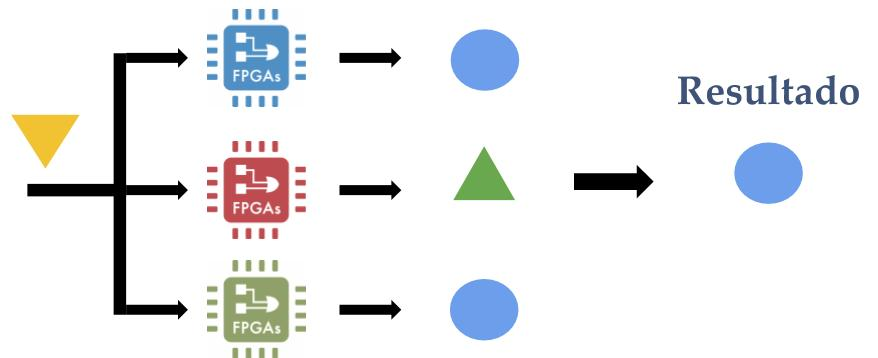
\includegraphics[scale=.45]{./Figures/Redundancia}
				\caption{Redundancia por votación 2 de 3.}
				\label{fig:Redundancia}
			\end{figure}
			
			También se ilustra en la Figura \ref{fig:Redundancia} el concepto de diversidad de plataformas de hardware, mediante las FPGA representadas en diferente color: azul, rojo y verde. Para mitigar fallos comunes a una misma plataforma de hardware o software una posible estrategia es utilizar sistemas de diferentes proveedores. %De esta forma, el resultado global es un sistema inmune a fallas singulares. No obstante, es vulnerable a fallas simultáneas de dos componentes, pero su probabilidad es mínima al ser de diferentes tecnologías u orígenes.
			
			%En este trabajo se implementó un sistema de enclavamiento electrónico, como se explicará en el Capítulo \ref{Chapter3}.

	\section{Objetivos}
	
		El objetivo de este proyecto fue el diseño, implementación y realización de pruebas funcionales de un prototipo de sistema electrónico de enclavamiento, sobre un kit de desarrollo de FPGA. 
		
		Se procuró además estudiar las tecnologías para implementar metodologías orientadas a mejorar los niveles RAMS del sistema, de acuerdo con el estado del arte en sistemas ferroviarios altamente críticos. 
		
		Teniendo la experiencia acumulada del trabajo realizado en la Especialización de Sistemas Embebidos, se puso especial énfasis en la automatización del proceso, para poder satisfacer las necesidades de cualquier locación. 

